\documentclass{beamer}
\usepackage{underscore}
\usepackage{color, german, graphicx}
\usepackage{eurosym}
\usepackage{fontenc}
\usepackage[utf8]{inputenc}
\usepackage{anyfontsize}
\usepackage{longtable}
\usepackage{mathptmx}
\usepackage{mathtools}
\usepackage{float}
\usepackage[backend=biber]{biblatex}
\addbibresource{report.bib}

\graphicspath{ {figures/} }
\restylefloat{figure}



\PassOptionsToPackage{demo}{graphicx}
\AtBeginSection[]
{
  \begin{frame}<beamer>
	\frametitle{Outline}
	\tableofcontents[currentsection]
  \end{frame}
}
\makeatletter
\newcommand\titlegraphicii[1]{\def\inserttitlegraphicii{#1}}
\titlegraphicii{}
\setbeamertemplate{title page}
{
  \vbox{}
   {\usebeamercolor[fg]{titlegraphic}\inserttitlegraphic\hfill\inserttitlegraphicii\par}
  \begin{centering}
    \begin{beamercolorbox}[sep=8pt,center]{institute}
      \usebeamerfont{institute}\insertinstitute
    \end{beamercolorbox}
    \begin{beamercolorbox}[sep=8pt,center]
      %\usebeamerfont{subtitle}
        \textbf{A\\ Stage One Dissertation Seminar On\\}
  	    \fontsize{14}{20}\selectfont \textbf{'Sentiment Analysis of transliterated hindi and marathi script'}\\
    \end{beamercolorbox}%
    \vskip1mm\par
    \begin{beamercolorbox}[sep=8pt,center]{author}
        By\\
      \textbf{Mr. Mohammed Arshad Ansari} (ME IT)\\
        Under the Guidance of \\
      \textbf{Prof. Sharvari Govilkar} 
    \end{beamercolorbox}
  \end{centering}
  %\vfill
}
\makeatother
\institute
{
    
\includegraphics[width=1cm]{piit.png}\\
	DEPARTMENT OF INFORMATION TECHNOLOGY\\
	PILLAIS INSTITUTE OF INFORMATION TECHNOLOGY\\
	ENGINEERING, MEDIA STUDIES AND RESEARCH\\
	NEW PANVEL - 410 206\\
	UNIVERSITY OF MUMBAI\\
	Academic Year 2015-16\\
}
 
\begin{document}

\begin{frame}[plain]
\maketitle
\end{frame}

% starting here

\section{Introduction}
    \frame{\frametitle{Introduction}
        \begin{itemize}
		    \item Presence of translited text in Literature
            \item Transliteration as vital source of sentiments
            \item Current state of affairs on the subject
            \item Why it matters now?
        \end{itemize}
    }

\section{Motivation}
    \frame{\frametitle{Motivation}
        \begin{itemize}
		    \item Reviews
		    \item Discourse Analysis
		    \item Feedback Analysis
            \item Other areas
        \end{itemize}
    }

\section{Literature Survey}
    \frame{\frametitle{Literature Survey} 
        \begin{longtable}[c]{ |p{5em}|p{5em}|p{5em}|p{5em}|p{5em}|  }
		\hline
        Paper & Author & Approach & Result & Limitation\\
		\hline
		\endhead
  Hindi subjective lexicon: A lexical resource for hindi poliarty
  classification \cite{bakliwal_hindi_2012} & Bakliwal, Akshat, Piyush Arora ad Vasudev Varma & Usage of
  sense based sentiment analysis and devlopment of HSWN& Resource for hindi &
  Doesn't work on transliteration of hindi text\\ 
        \hline
	    \end{longtable}
    }
    \frame{\frametitle{Literature Survey} 
        \begin{longtable}[c]{ |p{5em}|p{5em}|p{5em}|p{5em}|p{5em}|  }
		\hline
        Paper & Author & Approach & Result & Limitation\\
		\hline
		\endhead
  A framework for sentiment analysis in hindi using HSWN
  \cite{pandey_framework_2015} & Pooja Pandey , Sharvari Govilkar & Devnagiri
  sentiment analysis using HWSN
  and use of negation discourse analysis & Usage of negation and discourse
  analyse improves the result of polarity detection & Doesn't work with hindi
  transliteration\\
        \hline
	    \end{longtable}
    }
    \frame{\frametitle{Literature Survey} 
        \begin{longtable}[c]{ |p{5em}|p{5em}|p{5em}|p{5em}|p{5em}|  }
		\hline
        Paper & Author & Approach & Result & Limitation\\
		\hline
		\endhead
  Automatic Detection of English words in Benglish text: A statistical approach
  \cite{kundu_automatic_2012} & Kundu, Bijoy and Chandra, Swarup & Statistical
  method developed which is language independent and can be used to detect any
  foreign language. & Accuracy upto nearly 72 percent. & There is a great scope
  of increasing the accuracy by improving methodology.\\
        \hline
	    \end{longtable}
    }
    \frame{\frametitle{Literature Survey} 
        \begin{longtable}[c]{ |p{5em}|p{5em}|p{5em}|p{5em}|p{5em}|  }
		\hline
        Paper & Author & Approach & Result & Limitation\\
		\hline
		\endhead
  Sentiment Analysis of Hindi Review based on negation and discourse relation
  \cite{mittal_sentiment_2013} & Namita Mittal, Basant Agwarwal, Garvit Chouhan
  and Nitin Bania & Negation and discourse relation were identified and HSWN
  improvement carried out & Accuracy upto nearly 81 percent & Transl - iteration
  not covered. Scope for accuracy improvement.\\
        \hline
	    \end{longtable}
    }
    \frame{\frametitle{Literature Survey} 
        \begin{longtable}[c]{ |p{5em}|p{5em}|p{5em}|p{5em}|p{5em}|  }
		\hline
        Paper & Author & Approach & Result & Limitation\\
		\hline
		\endhead
  Text Normalization of Code Mix and Sentiment Analysis \cite{sharma_text_2015} & PYKL Sriniva and
  Shashank Sharma & Language identification and transliteration to devnagiri
  script and then using HSWN for sentiment analysis.& Accuracy upto 85 precent
  & Negation and discourse analysis not being performed. \\ 
  \hline
        \hline
	    \end{longtable}
	}
  
\section{Proposed Approach}
	\frame{\frametitle{Proposed Approach: Flow diagram}
        \begin{center}
            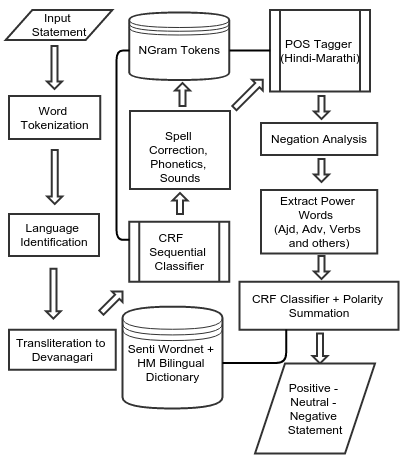
\includegraphics[width=60mm]{polarity-pickup.png}
        \end{center}
	}


    \frame{\frametitle{Proposed Approach}
	  \begin{enumerate}
            \item Text Normalization
		    \item NLP and Sentiment Analysis
	  \end{enumerate}
	}

    \frame{\frametitle{Proposed Approach - Text Normalization}
	  \begin{enumerate}
		\item Normalization Process for hindi
            \begin{enumerate}
                \item Spelling correction
                \item Ambiguous words
                \item Sounds
                \item Phontic words
                \item Transliteration
            \end{enumerate}
        \item Dictionary method for marathi using bilingual lexicon
	  \end{enumerate}
	}
    \frame{\frametitle{Proposed Approach - NLP and Sentiment Analysis}
	  \begin{enumerate}
		\item POS Tagging to identify nouns, adjectives and adverbs
            \begin{enumerate}
                \item Use machine learning to figure out POS for hindi
                \item In case of marathi, use bilingual dictionary and then tag the statement
            \end{enumerate}
		\item Adjective and Adverb extraction
            \begin{enumerate}
                \item Easier to do with POS tagged statements.
                \item If POS doesn't work, then use lexicon lookup
                \item Use senti wordnet or HSWN for looking up polarity count
                \item If lookup fails, use extended wordnet api for getting sense
            \end{enumerate}
        \item Negation and Classification using Classifier
            \begin{enumerate}
                \item Figureout negation in statements and then invert the POS tagged adjectives and adverbs
                \item Semi supervised naive bayes/svm classifier to classify the polarity - or -
                \item Simple summation of polarity will give a result to. Compare the two results
            \end{enumerate}
	  \end{enumerate}
	}

\frame{\frametitle{Proposed Approach: Algorithm for language identification}
\begin{longtable}[c]{ |p{11cm}|  }
  \hline
  \endhead
  \textbf{\textit{Arguments}} \\
  \hline
  w : word to identify language for\\
  sentence : sentence to which word belongs\\
  \hline
  if Leh is None:\\
  \hspace{4em}Leh = Qeh(Lh{i}) for i in Lh\\
  if Lem is None:\\
  \hspace{4em} Lem = Qem(Lm{i}) for i in Lm\\
    
  if not model:\\
  \hspace{4em}Model = CRF(FNGram(Leh), FNGram(Lem), FNGram(Le))\\
  \hspace{4em}if not w in D: \\
  \hspace{8em}w = stem word(w)\\
  \hspace{12em}if w not in D:\\
  \hspace{16em}w = find most similar word(D, w)\\
  l = arg max(Model, sentence, w)\\
  return l\\
  \hline
\end{longtable}
}

\frame{\frametitle{Algorithm for pos tagged with negetation}
\begin{longtable}[c]{ |p{11cm}|  }
  \hline
  \textbf{Algorithm steps} \\
  \hline
  \endhead
  if max(tags in sentence) is english:\\
  \hspace{4em}TaggedSentence = POSTaggerEnglish(sentence)\\
  else max(tags in sentence) is hindi:\\
  \hspace{4em}TaggedSentence = POSTaggerHindi(sentence)\\
  return replace negetive phrases with antonyms(TaggedSentence)\\
  \hline
\end{longtable}
}



\frame{\frametitle{Algorithm for polarity identification}

\begin{longtable}[c]{ |p{11cm}|  }
  \hline
  \textbf{Algorithm steps} \\
  \hline
  \endhead
  languageTaggedSentence = (LanguageIdentifier(sentence, word) for word in sentence).join(' ')\\
  posTaggedSentence = POSTag(languageTaggedSentence)\\
  polarWords = extractAdjectivesAdverbs(posTaggedSentence)\\
  wordPolarity = dict()\\
  for word in polarWords:\\
  \hspace{4em}if word tagged as english:\\
  \hspace{8em}wordPolarity[word] = sentiwordnetPolarity(word)\\
  \hspace{4em}elif word tagged as hindi:\\
  \hspace{8em}wordPolarity[word] = hindiSentiwordnetPolarity(word)\\
  \hspace{4em}else:\\
  \hspace{8em}hindiWword = hindiMarathiBilingualDictionary(word)\\
  \hspace{8em}wordPolarity[hindiWord] = hindiSentiwordnetPolarity(hindiWord)\\
  return wordPolarity\\
  \hline

\end{longtable}
}

\frame{\frametitle{Algorithm to classify polarity}
\begin{longtable}[c]{ |p{11cm}|  }
  \hline
  \textbf{Algorithm steps} \\
  \hline
  \endhead
  \textbf{\textit{Arguments}} \\
  \hline
  sentence : sentence to which word belongs\\
  \hline
  \textbf{\textit{Variables and methods}} \\
  \hline
  NaiveBayesClassifier -> Trained to return polarity of the entire sentence given tokens with polarity values\\
  LinearCalculation -> Simple Summation based polarity classifier\\
  \hline

  wordDictionary = PolarityIndentification(sentence)\\
  return NaiveBayesClassifier(wordDictionary), LinearCalculation(wordDictionary)\\
  \hline

\end{longtable}
}


\section{Application}
	\frame{\frametitle{Application}
	  \begin{enumerate}
		\item Reviews
		\item Discourse Analysis
		\item Feedback Analysis
        \item Other areas
	  \end{enumerate}
	}

\section{Conclusion}
	\frame{\frametitle{Conclusion}
	  \begin{enumerate}
		\item Accuracy of 95 percent on target
		\item Imporvement of transliteration sentiment analysis in general
        \item Usage of pre trained models over on the fly dynamic models for
            peformance gains
	  \end{enumerate}
	}


\section{Bibliography}
	\frame{\frametitle{References}}
    \printbibliography

\end{document}
